% TODO: Reformat citation and bibliography style, reformat paragraph spacing

\documentclass[12pt, english, openany]{book}

\usepackage[]{graphicx}
\usepackage[]{color}
\usepackage{alltt}
\usepackage[T1]{fontenc}
\usepackage[utf8]{inputenc}
\setcounter{secnumdepth}{3}
\setcounter{tocdepth}{3}
\setlength{\parskip}{\bigskipamount} % sets paragraph spacing
\setlength{\parindent}{0pt}

\usepackage[top=100pt,bottom=100pt,left=68pt,right=66pt]{geometry}
\geometry{a4paper}

\raggedbottom

\usepackage[english]{babel}

% All page numbers positioned at the bottom of the page
\usepackage{fancyhdr}
\fancyhf{} % clear all header and footers
\fancyfoot[C]{\thepage}
\renewcommand{\headrulewidth}{0pt} % remove the header rule
\pagestyle{fancy}

% Changes the style of chapter headings
\usepackage{titlesec}
\titleformat{\chapter}
   {\normalfont\LARGE\bfseries}{\thechapter.}{1em}{}
% Change distance between chapter header and text
\titlespacing{\chapter}{0pt}{25pt}{2\baselineskip}

% Adds table captions above the table per default
\usepackage{float}
\floatstyle{plaintop}
\restylefloat{table}

% Adds space between caption and table
\usepackage[tableposition=top]{caption}

% Adds hyperlinks to references and ToC
\usepackage{hyperref}
\hypersetup{hidelinks} % Changes the link color and hides the
% hideous red border that usually is created

% If multiple images are to be added, a folder (path) with all the images can
% be added here
\graphicspath{ {figures/} }

% Separates the first part of the report/thesis in Roman numerals
\frontmatter


\begin{document}
\selectlanguage{english}

\begin{titlepage}
	\clearpage\thispagestyle{empty}
	\centering
	\vspace{.5cm}

	% Titles
	{\large \textbf{Midterm Report} \par}
	\vspace{2.5cm}
	{\Huge \textbf{IPSTERS}} \\
  \vspace{1cm}
  {\Huge IPSentinel Terrestrial Enhanced Recognition System} \\
	\vspace{2.5cm}
	{\large \textbf{João Fonseca} \par}
	\vspace{.5cm}
	{\large \textbf{Advisor:} Prof. Fernando Lucas Bação, PhD \par}

	\vspace{1.5cm}
    
\includegraphics[scale=0.2]{ims_logo.png}
  \vspace{1.3cm}

	{\normalsize NOVA Information Management School \\
		Instituto Superior de Estatística e Gestão de Informação \\
		Universidade Nova de Lisboa \par}

  \vspace{1.5cm}

	% Set the date
	{\normalsize \textbf \today \par}
	\pagebreak
\end{titlepage}

\chapter*{Abstract}

This report documents the work developed towards the research project "IPSTERS
- IPSentinel Terrestrial Enhanced Recognition System". It focuses on the
exploration of several machine learning (ML) techniques, covering different
stages of a Land Use/Land Cover Classification (LULC) pipeline. These
techniques aim to minimise problems typically found in this kind of data,
namely data ingestion, feature selection, data filtering and classification.



\tableofcontents{}

\clearpage

\listoffigures

\clearpage

\listoftables

\mainmatter

\chapter{Introduction}

The Copernicus programme is the European Union (EU) Earth Observation (EO)
programme, headed by the European Space Agency, and the developer of the
Sentinels EO satellites. The IPSentinel is the Portuguese infrastructure
developed by Direção Geral do Território (DGT) and Instituto Português do Mar e
da Atmosfera (IPMA) for storing and providing images of Sentinel satellites,
covering the Portuguese territory and its search and rescue area. This free EO
data has been used to inform environmental models, business strategies and
political decisions. However, this ever growing volume of data requires big
data workload that is overwhelming for Public Administration (PA) agencies. As
a result, the use of IPSentinel data has not been widely adopted by the PA that
would profit from it.

Often what these agencies need for their goals are digested data in the form of
specific class maps. These value-added products are often called level-3
products and are fundamental for land-management and for the country's
international commitments such as the estimation of CO2 emissions. These
products are mainly obtained by visual interpretation of high resolution
satellite imagery, requiring significant allocation of human resources from the
PA and taking a long time to produce, being one of the reasons for the low
update rate and low resolution. In the case of COS (Portuguese Land cover-land
use maps) they are produced every 5 years with 1ha resolution and EU CORINE
maps at least every 6 years with 25ha.

\section{Purpose and Objectives}

The main goal of this project is to explore the applications and limitations of
artificial intelligence (AI) algorithms with accelerated processing hardware
capabilities, as a unit of the IPSentinel for the digestion of large volumes of
remotely sensed data, to produce level-3 products for land applications with
the least amount of human intervention. We propose exploring two artificial
intelligence approaches, one applying active learning techniques and another
based on fuzzy logic.
\\
Data used
\\
Code availability here
\\
Research grant info

\section{Document Structure}


\chapter{Literature Review}

The state of the art on the main challenges identified for the project is shown
here. The multispectral imagery used in this project is targeted for a large
area (continental Portugal) and contains complex and highly correlated spectral
information. Although the presence of multicollinearity doesn't pose a problem
for the adequacy of modern ML models to predict a target variable
\cite{Farrell2019}, high dimensional data is difficult to process and therefore
strains the capacity of producing accurate LULC maps. Dimensionality reduction
techniques are used to address such an issue. These techniques allow the
selection of the most important feature within the image composites used,
allowing for 1) a clearer understanding of the most important features for LULC
classification, 2) accelerated model training and 3) avert the curse of
dimensionality \cite{Ghojogh2019}.

% insert picture depicting data filtering vs feature selection vs feature extraction

% ask Arman for help on dataset description later on
The datasets used in this project are Sentinel 2 image composites overlaid with
the Portuguese Land cover-land use maps (COS). This
type of data is prone to noisy labelling for various reasons. Label noisy may
come from discrepancies between the original map's resolution (in the case of
COS, 1ha) and the objective map's resolution (for this project,
10m\textsuperscript{2}), as well as land cover type changes or classification
errors. % insert image with mislabeled regions
Mislabeled points are potentially problematic since the use of these points for
producing land cover maps at a 10m\textsuperscript{2} resolution can output
generalised and/or erroneous predictions. Therefore, it is necessary to
explore the need for noisy data filtering.

Finally, classification algorithms are discussed in the last section. These
algorithms should be resistant to noise and/or have correcting measures to
decrease the effect of the noisy data in the model's learning phase.

\section{Dimensionality Reduction Methods}
Dimensionality reduction techniques can be divided into 2 parts, feature
selection and feature extraction, both techniques explored below. Figure
\ref{fig:dimensionality-reduction} depicts the different types of techniques to
reduce a dataset's dimensionality.

\begin{figure}[H]
	\centering
	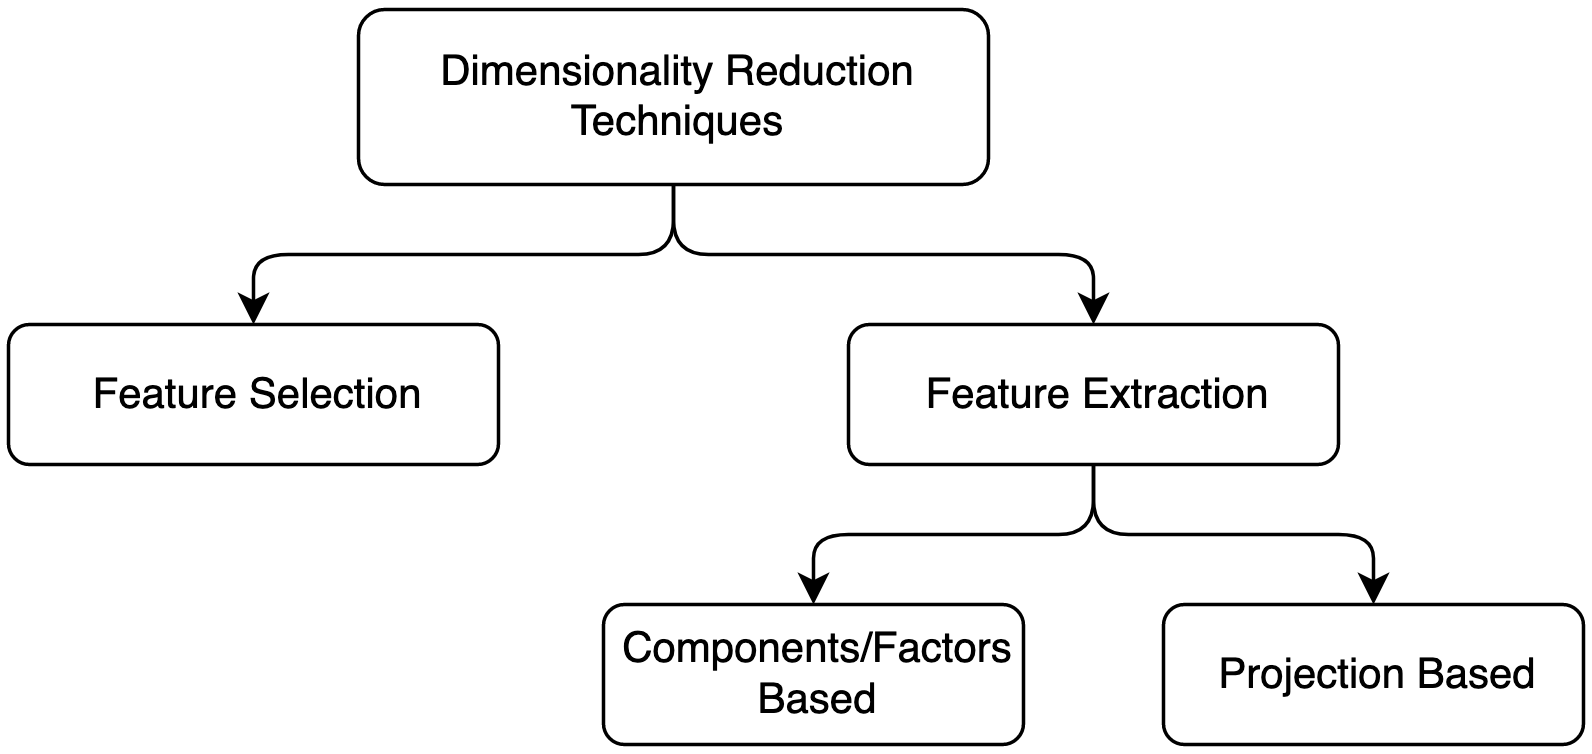
\includegraphics[width=.8\linewidth]{dimensionality_reduction.png}
  \caption{Dimensionality Reduction Techniques}
  \label{fig:dimensionality-reduction}
\end{figure}

Although all these methods reduce the dimensionality of data, the means used to
do so varies.

\subsection*{Feature Selection}

Feature selection methods reduce dimensionality through the selection of the
most important features among the ones already existing in the dataset. The
criterion used either improves, maintains the model accuracy, or simplifies the
model complexity. Below are presented commonly used supervise feature selection
methods. For more information on listed and/or additional methods the reader is
directed to \cite{Cai2018, Ghojogh2019}.

\begin{enumerate}
  % TODO: find references
  \item Correlation based feature selection (CFS). It's based on the predictive
  power of a feature subset, found by computing the correlation between the
  feature subset and the target feature. It is therefore a generalisation
  of the Correlation Criteria as defined in \cite{Ghojogh2019}.
  \item ReliefF \cite{kononenko1997}. It's an extension of Relief
  \cite{kira1992} to support multi-class problems. For each instance, the
  algorithm considers the closest instance from each class to update the
  feature score vector. The score of any given feature decreases if it differs
  more in nearby instances of the same class than nearby instances of the other
  class, and increases in the reverse case.
  % TODO: Find references
  \item Random Subspace Method (RSM) and Random Forest Method (RFM). Consists
  in the training of base classifiers on different feature subsets. These
  methods use the trained classifiers to assess each feature's importance to
  the prediction of the target variable. In the case of RFM, it is important to
  consider that Tree based classifiers are trained through the minimisation of
  entropy on each data split. As such, variables used earlier for decision
  rules along a decision tree's path is deemed as having a higher importance
  than the remaining variables.
\end{enumerate}

% TODO: Find references
Along with the presented methods, a number of variations are being applied by
practitioners, such as Permutation Feature Importance (shuffling each feature
after training a classifier and check accuracy drops) and Drop Column Feature
Importance (dropping one feature and checking differences in accuracy compared
to a classifier using all available features).


\subsection*{Feature Extraction}
TODO


\section{Data Filtering Methods}

The accuracy of a classifier is directly affected by the quality the training
data used \cite{Boukir2019}. Despite the importance of classification tasks in
remote sensing, obtaining well-labelled data is time consuming, impracticable
and expensive \cite{Pelletier2017Filtering}. To the best of our knowledge there
is no systematic review on data selection/filtering methods for the remote
sensing domain. Through the analysis of the different algorithms available, 2
distinct types of filtering were identified, each dividing into 2 subgroups.
Figure \ref{fig:noisy-label-detection} depicts the different methods found for
this purpose.

\begin{figure}[H]
	\centering
	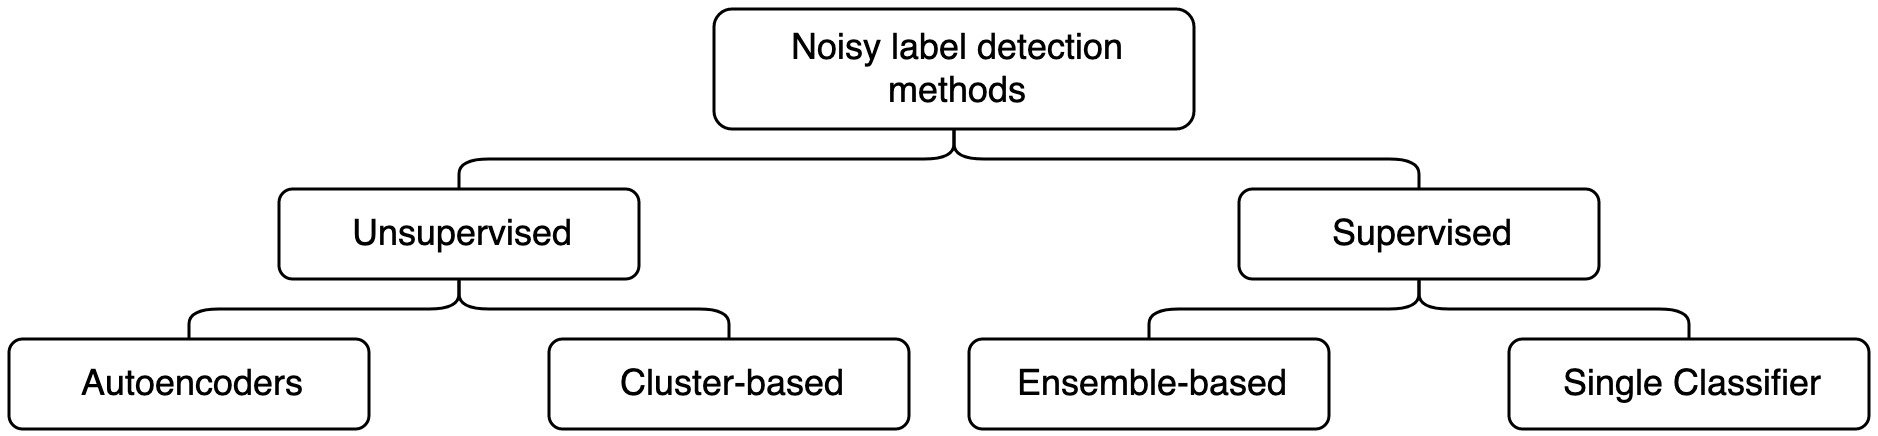
\includegraphics[width=1\linewidth]{noisy_label_detection.png}
  \caption{Different types of methods found for noisy label detection.}
  \label{fig:noisy-label-detection}
\end{figure}

LULC maps are commonly presented in a shapefile format. A recent study
employed polygon membership information for each pixel to detect labelling
errors within each polygon. This was done through the use of clustering methods
and cross cluster consistency measurement methods \cite{Paris2019}. Variations
on this method are explored and documented below.

A frequent type of approach to address this challenge is based on the use of
different machine learning classifiers to detect these errors
\cite{Brodley1999, Jiang2004, Liu2008, Yuan2018, Zhang2018,
Pelletier2017Filtering, Garcia-Gil2019, Boukir2019, Zhang2019}. These methods
benefit from classifiers' specificities, especially Random Forest, to implement
different voting strategies and model fitting methods to improve label noise
detection. Since these methods don't use domain specific information, they can
be used over any machine learning problem.

Although the impact of these filtering methods on robust classifiers is
unknown, some studies document the impact of label noise on classification
accuracy, showing the robustness of Random Forests and Deep Learning algorithms
\cite{Pelletier2017Effect, Rolnick2017}. Relevant filtering methods presented
in this section will incorporate the experiment, where the impact of data
filtering can be assessed (although these results are accompanied with
significant limitations).

% In order to add an unnumbered section/chapter:
%\addcontentsline{toc}{section}{Uppgift 1}
\subsection*{Unsupervised methods}

The best performing label noise detection algorithm based on clustering methods
was proposed by \cite{Paris2019}. This method assumes the availability of a
LULC map provided at a polygon level. The training set identification method is
based on 3 steps:
\begin{enumerate}
  \item Polygon k-means clustering. Starts by clustering the points within each
  separate polygon using the K-Means clustering algorithm and the Calinski
  Harabasz index (CHi) to automatically determine the optimal number of
  clusters for each polygon. The majority cluster of each polygon passes on to
  the next step, while all pixels belonging to the minority clusters are
  dropped and disregarded for potential training set candidates. Figure
  \ref{fig:paris-kmeans} depicts a qualitative example of this step.

  \item Polygon consistency analysis. Majority clusters are submitted to
  consistency analysis, which is done by computing each cluster's Bhattacharyya
  distance (B-distance) to compute the similarity of each subset to the entire
  set of clusters of the corresponding class. Afterwards, the clusters with
  distance from the entire set of clusters smaller than the
  65\textsuperscript{th} percentile of the cluster distances are selected for
  Stratified Random Sampling.

  \item Stratified Random Sampling. This step ensures the generation of a
  balanced dataset, proportionate to the original class ratios.
\end{enumerate}

\begin{figure}[H]
	\centering
	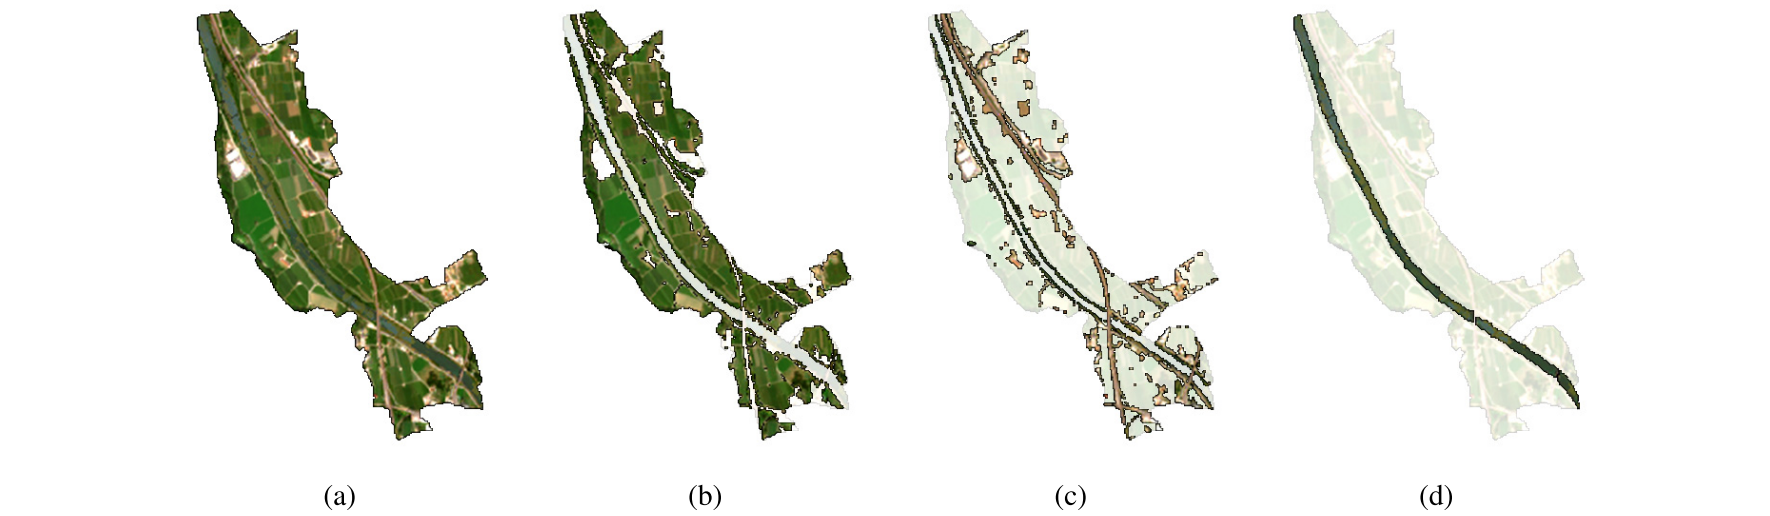
\includegraphics[width=1\linewidth]{paris_kmeans_results.png}
  \caption[Qualitative example of polygon k-means clustering
  result.]{Qualitative example of polygon k-means clustering result. (a)
  Original polygon associated to the “crop” label. (b) Dominant land-cover
  class detected C1. (c) First minor class detected C2 (road). (d) Second minor
  class detected C3 (river). Source: \cite{Paris2019}}
  \label{fig:paris-kmeans}
\end{figure}

Through qualitative analysis, this method achieved satisfactory results.
Regardless, it is difficult to determine the quality of these
results without reference data.

Other approaches include the use of autoencoders. Each class is used to train
an autoencoder, allowing the models to learn how to make latent representations
of instances belonging to a single class. For each instance, a reconstruction
error will be computed, using it as the mislabel score (the higher the error,
the more likely the instance is mislabeled) \cite{Zhang2019}.


\subsection*{Supervised methods}

All supervised methods take a quantitative approach to the problem.
Typically, these methods minimise either one of two errors. On the one hand,
instances incorrectly tagged as mislabeled represent an E1 error. On the other
hand, mislabeled instances left untagged represent an E2 error. Figure
\ref{fig:types-detection-errors} shows a visual representation of the two types
of error.

\begin{figure}[H]
	\centering
	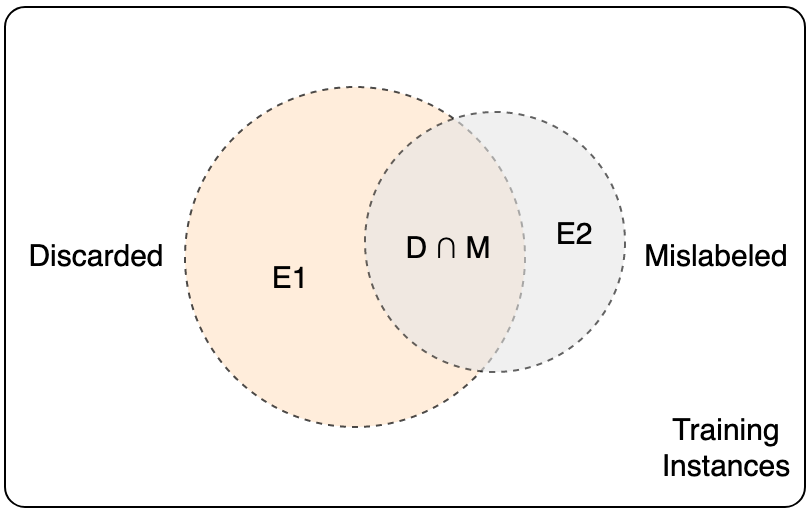
\includegraphics[width=.6\linewidth]{detection_errors_types.png}
  \caption[Types of detection errors.]{Types of detection errors. Adapted from
  \cite{Brodley1999}.}
  \label{fig:types-detection-errors}
\end{figure}

Supervised methods can be divided into 2 subgroups:
\begin{enumerate}
  \item Single model approaches. They use a single model to determine wether a
  specific instance is correctly labelled. A common implementation includes the
  use of a standard classifier to predict the label of an instance and tagging
  it as mislabeled if the classifier's prediction differs from the original
  label \cite{Brodley1999}.
  \item Ensemble-based approaches. They use a set of weak classifiers (most
  commonly Decision Trees) to generate a number of output predictions. These
  classifiers are always trained in a subset of the dataset, which are then
  used to predict the label of the remaining dataset. Consequently, this set of
  classifiers is trained $k$ times, depending on the number of splits used in
  the data stratification. These predictions are then changed to a binary
  output of correct/incorrect prediction according to the original label. The
  more incorrect predictions over a single instance there are, the more likely
  it is for it to be tagged as mislabeled. The methods for aggregation of the
  set of individual votes to compute the final score differ according to the
  method used.
\end{enumerate}

Single model approaches benefit from reduced computation power and generally
improve the quality of the training set generated, although they rarely
outperform any ensemble-based approach \cite{Brodley1999, Garcia-Gil2019,
Boukir2019, Pelletier2017Filtering, Zhang2018, Yuan2018}.

Within ensemble-based approaches there is a simple underlying calculation of a
mislabel likelihood (henceforth referred to as mislabel ratio). For traditional
methods the calculation consists in a simple ratio between the count of
incorrect prediction over the total number of predictions:
\begin{equation} \label{eq:mislabel-ratio}
  MR(x) = \frac{n-\sum_{i=1}^{n}{v_i^y}}{n}
\end{equation}
Where $n$ is the number of predictions for an instance $x$ and $v_i^y$ is 0 if
the predicted label differs from the true label, 1 otherwise. Although any
threshold could be set for $MR$ in order to consider an instance's label
incorrect, most of the literature uses 2 different thresholds, referred to as
consensus ($MR=1$, i.e., all predictors fail to classify an instance's true
label) and majority filtering ($MR\geq0.5$, i.e., the majority of predictors
fail to classify an instance's true label). Therefore, consensus filters focus
on the minimisation of E1 error whilst majority filtering minimises E2 error
\cite{Brodley1999, Yuan2018}. Other methods have been used to measure mislabel
likelihood. \cite{Boukir2019} proposed an ensemble margin score, defined as:
\begin{equation} \label{eq:ensemble-margin}
  EM(x) = \frac{2\sum_{i=1}^{n}{v_i^y}-n}{n-\sum_{i=1}^{n}{v_i^y}}
\end{equation}

Both majority and consensus filtering have been used in a number of recent
publications \cite{Garcia-Gil2019, Boukir2019, Pelletier2017Filtering,
Zhang2018, Yuan2018}. Some of these methods \cite{Boukir2019, Yuan2018}
achieved improved performance by implementing an iterative approach to the
problem, consisting in multiple applications of filtering process a dataset,
gradually reducing its size on each iteration. Figure
\ref{fig:ensemble-filter-pipeline} provides a visual representation of an
ensemble-based filtering pipeline.

\begin{figure}[H]
	\centering
	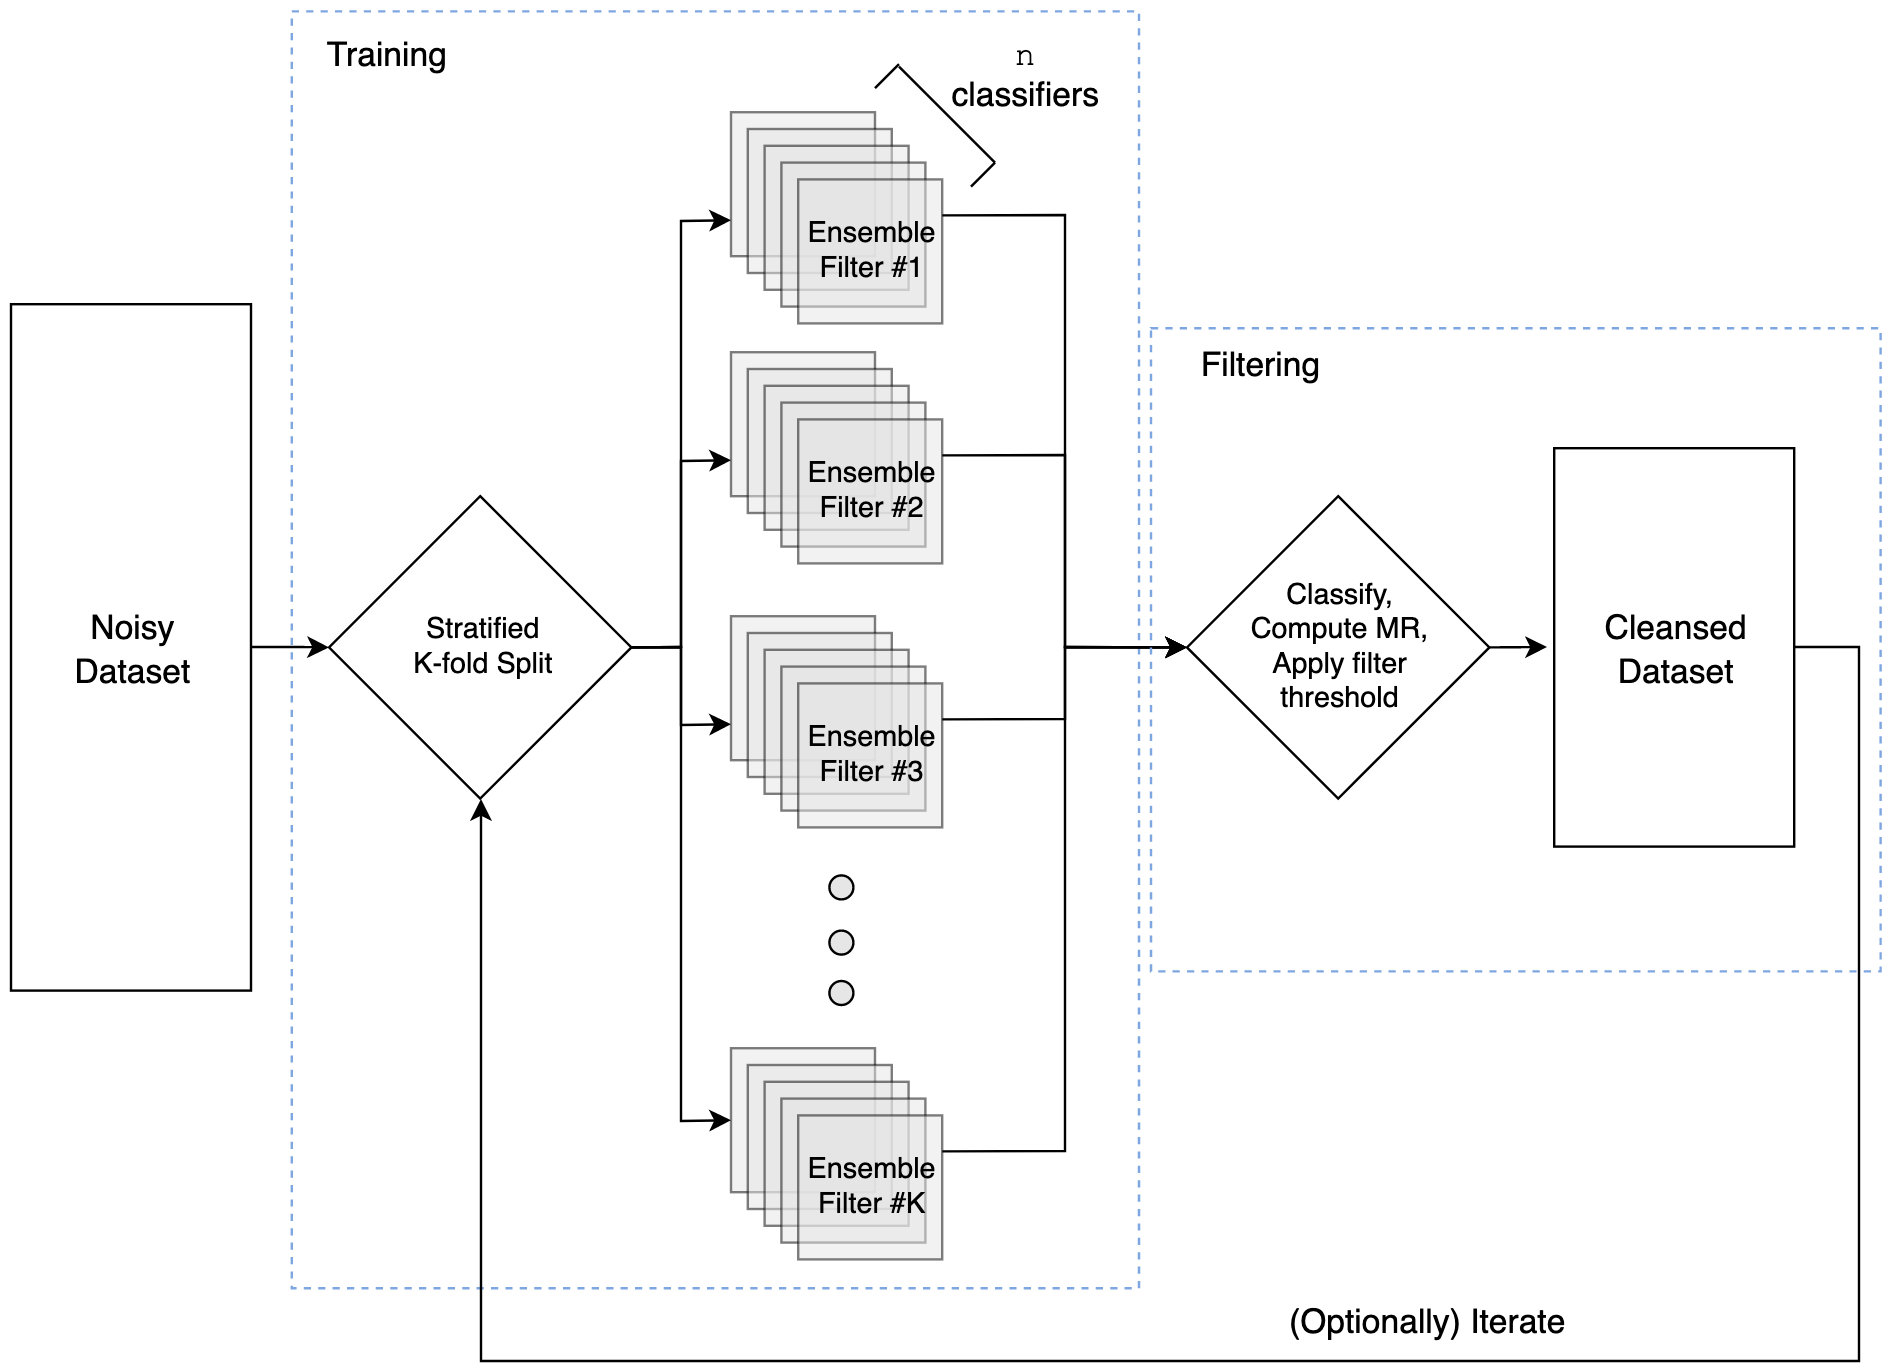
\includegraphics[width=1\linewidth]{enfilter_pipeline.png}
  \caption{Ensemble-based approaches pipeline.}
  \label{fig:ensemble-filter-pipeline}
\end{figure}

Isolation Forest (iForest) \cite{Liu2008} is another common method used for
data filtering. It benefits from the use of a set of Isolation Trees (iTrees)
that attempt to isolate each instance within the dataset. The rationale behind
this algorithm consists in the measurement of the average path length an
instance goes through in all iTrees, assuming that an anomaly (in this case, a
mislabeled instance) has a different profiles than that of the remaining
population of the corresponding label. Consequently, a mislabelled instance is
expected to have a smaller path length than that of a correctly classified
instance, as demonstrated in Figure \ref{fig:iforest-demonstration}.

\begin{figure}[H]
	\centering
	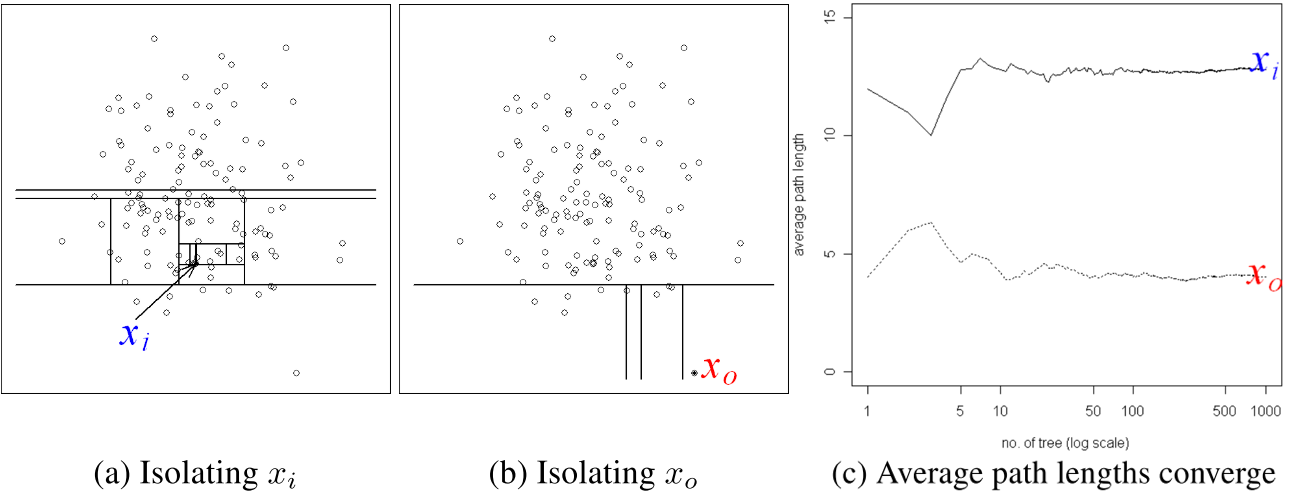
\includegraphics[width=1\linewidth]{iforest_demo.png}
  \caption[Anomaly detection using the iForest algorithm.]{Anomaly detection
  using the iForest algorithm. Anomalies are more susceptible to isolation and
  hence have short path lengths. (a) a normal point $x_i$ requires twelve
  random partitions to be isolated; (b) an anomaly $x_o$ requires only four
  partitions to be isolated. (c) averaged path lengths of $x_i$ and $x_o$
  converge when the number of trees increases. Source: \cite{Liu2008}}
  \label{fig:iforest-demonstration}
\end{figure}



\section{Classification Methods}

The most common classifiers identified for land cover image classification are
Random Forests (RFC), Support Vector Machines (SVM), K-Nearest Neighbours
(KNN), artificial neural networks (ANN), Maximum Likelihood (ML) and Decision
Trees (DT) \cite{Khatami2016, Maxwell2018}. However, recent literature has
focused on the implementation of robust classifiers such as Convolutional
Neural Networks with varying structures, Random Forests and Autoencoders
\cite{Roy2019, Zhang2017, Li2016}.

\subsection*{Convolutional Neural Networks}
TODO

Hybrid Spectral Net

ResNet

\subsection*{Random Forests}
TODO

\subsection*{Autoencoders}
TODO

\chapter{Methodology}

This chapter describes the work developed so far, along with the models implemented for each phase the pipeline that will ultimately produce an algorithm able to output an accurate LULC map.

The implementation of the experimental procedure was based on the Python programming language, all functions, algorithms, experiments, and results reported are available in the project's \textcolor{blue}{\href{https://github.com/joaopfonseca/remote_sensing}{Github repository}}.

\section{Datasets}

\section{Preprocessing}

\subsection{Dimensionality Reduction}

\subsection{Data Filtering}

\section{Classification}

\section{Experiment Settings}

\chapter{Results and Discussion}



% Adding a bibliography if citations are used in the report
\bibliographystyle{plain}
\bibliography{references.bib}
% Adds reference to the Bibliography in the ToC
\addcontentsline{toc}{chapter}{\bibname}


\end{document}
